
%%%%%%%%%%%%%%%%%%%%%%% file typeinst.tex %%%%%%%%%%%%%%%%%%%%%%%%%
%
% This is the LaTeX source for the instructions to authors using
% the LaTeX document class 'llncs.cls' for contributions to
% the Lecture Notes in Computer Sciences series.
% http://www.springer.com/lncs       Springer Heidelberg 2006/05/04
%
% It may be used as a template for your own input - copy it
% to a new file with a new name and use it as the basis
% for your article.
%
% NB: the document class 'llncs' has its own and detailed documentation, see
% ftp://ftp.springer.de/data/pubftp/pub/tex/latex/llncs/latex2e/llncsdoc.pdf
%
%%%%%%%%%%%%%%%%%%%%%%%%%%%%%%%%%%%%%%%%%%%%%%%%%%%%%%%%%%%%%%%%%%%


\documentclass[runningheads,a4paper]{llncs}

\usepackage{amssymb}
\setcounter{tocdepth}{3}
\usepackage{graphicx}
\usepackage{cite}
\usepackage{url}
\usepackage{natbib}
\usepackage{etoolbox}
\urldef{\mailsa}\path|{samuel.neaves, sophia.tsoka}@kcl.ac.uk|


\renewcommand{\bibname}{\leftline{References}}
   
\newcommand{\keywords}[1]{\par\addvspace\baselineskip
\noindent\keywordname\enspace\ignorespaces#1}

\begin{document}

\mainmatter  % start of an individual contribution

%
\title{Using ILP to Identify Pathway Activation Patterns in Systems Biology}
% oe Identifying Pathway Activation Patterns- For Classification
%ILP identifies pathway activation patterns. 
%n Application of ILP to Systems Biology
% a short form should be given in case it is too long for the running head
\titlerunning{Using ILP to Identify Pathway Activation Patterns in Systems Biology}

% the name(s) of the author(s) follow(s) next
%
% NB: Chinese authors should write their first names(s) in front of
% their surnames. This ensures that the names appear correctly in
% the running heads and the author index.
%
\author{Samuel R Neaves, Dr Sophia Tsoka}
%
\authorrunning{Using ILP to Identify Pathway Activation Patterns in Systems Biology}
% (feature abused for this document to repeat the title also on left hand pages)

% the affiliations are given next; don't give your e-mail address
% unless you accept that it will be published
\institute{Department of Informatics King's College London,\\
Strand, London, UK\\
\mailsa\\
%\mailsc\\
\url{http://www.kcl.ac.uk}}

%
% NB: a more complex sample for affiliations and the mapping to the
% corresponding authors can be found in the file "llncs.dem"
% (search for the string "\mainmatter" where a contribution starts).
% "llncs.dem" accompanies the document class "llncs.cls".
%

\toctitle{Using ILP to Identify Pathway Activation Patterns in Systems Biology}
\tocauthor{Samuel R Neaves}
\maketitle


\begin{abstract}
We show a logical aggregation method that, combined with
propositionalization methods, can construct novel structured biological
features from gene expression data. We do this to gain understanding of pathway
mechanisms, for instance those associated with a particular disease.

\keywords{ILP, Biological pathways, Warmr, Treeliker, Reactome, Barcode, Logical aggregation, RDF.}
\end{abstract}



\section{Introduction and Background}

%This paper describes a method to use Inductive Logic Programming(ILP) techniques to mine structured biological data. 
%Overview
In the field of Systems Biology researchers are often interested in identifying perturbations within a biological system that are different across experimental conditions. In this paper we use the example of identifying differences in perturbations between two types of Lung Cancer.
%To clarify we are looking to identify differences rather than building a diagnostic tool for Lung Cancer.

% typical approach
A typical pipeline for this kind of task has three distinct stages. The first stage is to use a technology such as a microarray or RNAseq to measure gene expression across the genome in a number of samples from each of the experimental conditions. 
The second stage is to identify a subset of genes whose expression values differ across conditions.
This stage is commonly achieved by performing differential expression analysis and ranking genes by a statistic such as fold change values. A statistical test is then used to identify the relevant set to take forward to stage 3. 
Alternatively for stage 2 researchers may train a model using machine learning to classify samples into experimental conditions, often using an attribute value representation where the features are a vector of gene expression values. 
This approach has the advantage that the constructed model may have found dependencies between genes which would not have been identified otherwise.
%(experimental conditions). 
Researchers will use the \lq top\rq\ features from the model to identify the set of genes to take on to stage 3. 
%Genes that are identified in this manner may be  different to a simple list of differently expressed genes as the constructed model , which are not highly differently expressed. 


%We note classification is often not the true task -the classification performance is used as a measure of the quality of the identified differences. Classification might not be the true task as the class of a sample may already be known - for example where the biopsy is taken from may indicate the class. 
%typical approach stage 2
In stage 3  researchers look for connections between these genes, for example by performing Gene Set Enrichment Analysis (GSEA) \citep{subramanian_gene_2005}. Here the set of genes identified in stage 2 are compared with predefined sets of genes. Each predefined set of genes indicate a known relation. For example having a related function, existing in the same location in the cell or taking part in the same pathway. 

%related relational work
To bring background knowledge of relations into the model building process, past ILP research \citep{gamberger_induction_2004} integrated stage 2: finding differentially expressed genes and stage 3: GSEA, into a single step. This was achieved using Relational Subgroup Discovery, which has the advantage of being able to construct novel sets by sharing variables across predicates that define the sets. For example a set could be defined as the genes that have been annotated with two Gene Ontology terms.  

Other ways researchers have tried to integrate the use of known relations is by adapting the classification approach. New features are built by aggregating across a predefined set of genes - for example by taking an average expression value for a pathway, see ~\citep{holec_comparative_2012} for a review of these methods.
A major limitation of current classification approaches is that the models are constructed from either genes or crude aggregates of sets of genes, and so ignore the detailed relations between entities in a pathway. 
In order to incorporate more complex relations a network representation is needed.
It is important that this representation is appropriate such that biological relations are adequately represented.
For example a simple directed network of genes and proteins does not adequately represent the complexities of biochemical pathways such as the dependencies of biochemical reactions. To do this bipartite graphs or hypergraphs can be used (see \citep{whelan2011representation} for more details). 

One way to incorporate more complex relations is by creating topologically defined sets, for example by performing community detection in a gene regulatory network.
However, this approach can create crude clusters of genes, that do not account for important known biological concepts.
Biologists are also interested in complex biological interactions rather than just sets of genes, as we now describe. 


Network motif and frequent subgroup mining  \citep{kim_biological_2011} are methods that can look for structured patterns in biological networks. However, in these approaches the patterns are often described in a language which is not as expressive as first order logic. This means they are unable to find patterns with uninstantiated variables, or with relational concepts such as paths or loops.
%It is also the case that motifs or frequent subgraphs are rarely identified for the purpose of discrimination in a classification task.
For example, in Figure~\ref{fig1}a we show a toy example of four instantiations of the same graph, three in class A and 1 in class B.
A frequent pattern distinguishing between the classes may be a chain of three on reactions. 
This may be represented in Prolog as \emph{on(a),on(X),on(c),link(a,X),link(X,c)}. However, 
network motif finding can only work with  patterns such as \emph{$a_{on} \rightarrow b_{on} \rightarrow c_{on}$}, and hence would not be able to find the repeated pattern. 


\begin{figure}
\centering
   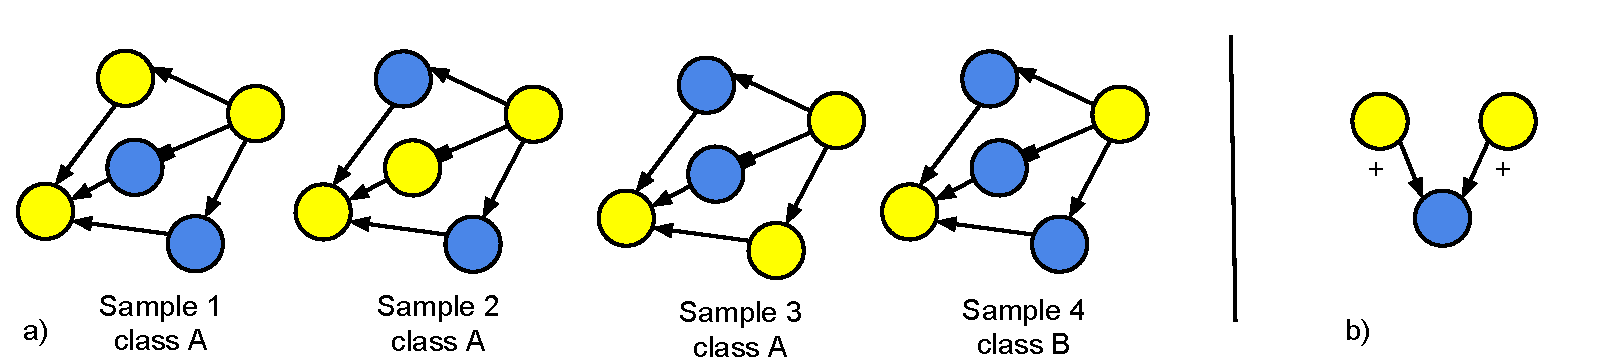
\includegraphics[width=0.8\textwidth]{graph.pdf}
   \caption{Example graphs. Node color indicates expression activity. Yellow: on; blue: off.}
   \label{fig1}
\end{figure}


To our knowledge only one previous work has looked to use ILP for this task \citep{holec2008using}.
Here the authors propose identifying features consisting of the longest possible chain of vertices in which non-zero vertex activation implies a certain (non-zero) activation in its successors, which they call a Fully Coupled Flux.

%using Fully Coupled Fluxes (FCF) as features. 

The aim of this paper is to identify pathway activation patterns that differ between biological samples of different classes, in order to give a biologist different information than models built from simple gene features.

An example of when such a pattern is useful is in consistency modelling \citep{guziolowski2010analysis}.
Here a pattern of inconsistency, an example of which is given in Figure~\ref{fig1}b, is matched against gene regulatory networks. 
Then for each match Answer Set Programming techniques are used to amend the pathways and remove the inconsistency. Similar work has been carried out in ILP  where biological pathways have been constructed and amended \citep{ray2010automatic}.
The patterns identified with our approach could be used in a similar task to further understand the system level perturbations between classes.

%In contrast to the work on consistency modelling but consistent with the FCF approach, we assume the pathways are an accurate representation of biological processes and we are considering individual sample expression values mapped on to the pathway. 

%Network represenation

%In consistency modelling \citep{guziolowski2010analysis} a pattern of inconsistency is matched against gene regulatory networks and for each match Answer Set Programming techniques are used to amend the pathways to remove the inconsistency. Similar work has been carried out in ILP  where biological pathways have been constructed and amended \citep{ray2010automatic}. 

% including paths and loops where some of the entities could possibly be represented by uninstantiated variables. 
%For example, these are used in Consistency modelling a method where ... 
%

%Network motif finding is a set of methods to find general patterns. 




%Most motif finding algorithms are applied to a network representation which is inappropriate for pathways. There is also a failure to adapt the motif finding algorithm to take into account biological knowledge.   Motifs are most commonly searched for across a single network constructed from an agglomerative of the experimental data, rather than by mapping expression values to a standard graph of the pathway. This approach would give an instantiated graph for each sample and enables the searching for pathway activation patterns (using the node states) across samples - taking into account the class of each sample. 
 
%\section{Aim}
%

	  
\section{Methods}
 We use structural pathway information to build first order features that are used to construct classification models that discriminate between two lung cancer types.
 We collate raw data from online sources, process this data to create a
 Prolog knowledge base, and then learn first order models using this knowledge base. 

\subsection{Raw Data} 
We obtained from the GEO a two class Lung Cancer data set containing 37 SCC examples and 33 AC examples; the accession number is GSE2109.The classes correspond to different types of Lung Cancer. For details of this task please see \citep{rhrissorrakrai_sbv_2013}.  
We use the Reactome database to provide the background knowledge about pathways. Reactome \citep{croft_reactome_2013} is a collection of manually curated peer reviewed pathways. Reactome is made available as an RDF XML Biopax level 3 file file, which allows for simple passing using SWI-Prolog's semantic web libraries. 


\subsection{Data Processing}
Reactome uses the bipartite network representation of entities and reactions. 
We extract and process this to create a reaction centric graph, where nodes are reactions and directed edges are labelled either as \lq activation\rq\ ,\lq inhibition \rq\ or \lq follows\rq\ corresponding to how reactions are connected. 
Boolean networks~\citep{wang_boolean_2012} are a common abstraction in biological research, but these are normally applied at the gene or protein level not at the reaction level. In order to use a boolean network abstraction on a reaction network, we apply a logical aggregation method that aggregrates measured probe values in the microarray into reactions.

The first step of this aggregation is the discretization of the probe values into binary values. 
We do this using Barcode \citep{mccall_gene_2014}, a tool for converting the continuous probe values to binary variables by applying previously learnt thresholds to microarray data. 
This makes it possible to compare gene expressions, both within a sample and between samples potentially measured by different arrays. 

Once we have binary probe values, we use the structure provided by
the Reactome RDF graph and key biological concepts to build reaction level features. 
Each reaction has a set of inputs that are required for a particular reaction. In addition a reaction may be controlled (activated or inhibited) by particular entities. 
Entities in Reactome include protein complexes and protein sets, which can themselves comprise of other complexes or sets. 
We interpret each reaction input as a logical circuit. The relationship between probes and proteins is treated as an OR gate, protein complexes as an AND gate, and protein sets also as an OR gate. 
A final step takes into account the activation or inhibition of the reaction by any controlling entities. 
In this way we can say that a reaction \lq can proceed\rq\ if and only if the input circuit evaluates to true. 
If a reaction \lq can proceed\rq\ then we say that it is \lq on\rq\ otherwise we say that it is \lq off\rq. %In this way we have created a biologically informed aggregate set of features at the reaction level, which has used the internal structure of a pathway in their construction. 

\subsection{Searching for Pathway Activation Patterns}
We experimented with two propositionalization methods, Warmr and Treeliker, separately and then combining them. We search for features independently in each pathway and with a language bias that suitably constrains the search in order to achieve a manageable number of structures. 

The first method, Warmr \citep{dehaspe_mining_1997}, is the first order equivalent of item set and association rule mining. It can be used as a propositionalization method by independently searching for frequent queries in the two classes. An advantage of Warmr is that it is possible to define background predicates for relevant concepts. For example a path or loop of all \lq on\rq\ reactions. As Warmr does not prune by relevance to classification tasks it can however quickly build to an intractable search with many irrelevant or similar queries/features built. 

The second method, TreeLiker~\citep{vzelezny2013fast}, is a modern ILP tool that implements a number of algorithms. It has been shown to produce long features by building features bottom up in a blockwise manner. This is desirable for our task as longer features will provide more mechanistic insight to a biologist. A limitation is that the features are \lq tree like \rq\ which means there can be no cycles in the variables. Unlike Warmr, TreeLiker does not support explicit background knowledge and therefore all relevant relations need to be preprocessed using Prolog.

Our combined method takes a top feature constructed by TreeLiker and uses this as the basis for the language bias input into Warmr. 
We then add language bias constraints that guide Warmr to add cycles to the tree like feature.
This results in long cyclical features that Warmr would not be able to find on its own. 
	     
To evaluate the generated features we use them to build classifiers, to estimate their ability to discriminate between the two lung cancer types.
We use the J48 and JRIP tree and rule building algorithms of the Weka package to do this, chosen because these produce interpretable models.

\section{Preliminary Results}
%As we are interested in producing comprehensible models, we limit our experiments to rule (JRIP) and tree building algorithms (J48).We employ Wekas implementation. 

We give the following example features found by 1) Warmr, 2) TreeLiker and 3) our combined approach:
\begin{verbatim}
1:array(A),reaction(A,B,1),reaction(A,C,0),link(C,B,D),link(B,C,E).
\end{verbatim}

\begin{verbatim}
2:reaction(A,0), link(A,B,follows), reaction(B,1), link(B,C,_),    
reaction(C,0), link(A,D,activation), reaction(D,0).
\end{verbatim}

\begin{verbatim}
3:array(A),reaction(A,B,0),link(B,C,follows),reaction(A,C,1),
link(C,D,E),reaction(A,D,0),link(B,F,activation),reaction(A,F,1),
link(F,D,E),link(D,G,E),reaction(A,G,0)
\end{verbatim}
\noindent
Feature 1 is a simple cyclical feature found by Warmr, the variable A matches one sample. 
Feature 2 is a longer tree like feature found by TreeLiker. Notice TreeLiker does not require a variable for the sample.  
Feature 3 is found by our combined method, it is both long and contains a cycle. 


To date we have found promising features for the Apoptosis pathway, which, using  
the Jrip model, achieved mean 81.29\% accuracy (std 13\%) using 10 fold cross validation. This is a comparable accuracy to that of a model built with raw expression values, but now we have identified pathway activation 
perturbations rather than just gene expression perturbations. 


\section{Discussion}
The Pathway Activation Patterns we found using this approach are in clinically relevant pathways. These patterns may give diagnostic and clinical insights that biologists can develop into new hypotheses for further investigation. 

This work has shown the potential of ILP methods for mining the abundance of highly structured biological data. Using this method we have identified differences in Pathway Activation Patterns that go beyond the standard analysis of differentially expressed genes, enrichment analysis, gene feature ranking and pattern mining for common network motifs. We have also demonstrated the use of logical aggregation with a reaction graph and how this simplifies the search for hypotheses to an extent where searching all pathways is tractable. 
We have introduced a novel approach that uses Warmr to extend features initially identified with TreeLiker. This makes it possible to search for long cyclical features. 
\newline


%\subsubsection*{Acknowledgments.} Thanks to ...


\begingroup

\makeatletter
\patchcmd{\@makeschapterhead}{\vskip40}{\vskip12}{}{} 
\makeatother

\let\clearpage\relax
\bibliography{mybib}{}
\endgroup

%\bibliography{mybib}{}
%\bibliographystyle{plain}
\bibliographystyle{unsrt}
%\bibliographystyle{unsrtnat}
%\bibliographystyle{ieeetr}





\end{document}
